\textcolor{secundario}{VALOR ACTUAL INTERNO.} Se llev\'o a cabo la valuaci\'on del capital intangible a partir de la informaci\'on de negocio y financiera proporcionada por el solicitante, habiendo aplicado el marco te\'orico de la valuaci\'on de negocios; bajo el punto 2 del pent\'agono de McKinsey (Value as is\footnote{Valor Actual Interno} ): (\textcolor{terciario}{\autoref{fig:hexagono}}).

\begin{figure}[H]
\centering
\caption{Pent\'agono de Explotaci\'on de oportunidades\label{fig:hexagono}}
\includegraphics[width=9cm]{\rutaImagenes/pentagono}\\
Fuente:Valuation. Copeland Tom, Koller Tim y Murrin Jack.\\

John Wiley \& Sons. 2000.
\end{figure}

``\textcolor{secundario}{Valor en las condiciones actuales.} Es el valor de la unidad econ\'omica valuado en las condiciones que opera al d\'ia de hoy, esto es, sin realizar ninguna explotaci\'on de oportunidades en los factores internos y externos. Este valor resulta de la aplicaci\'on de un trabajo valuatorio para determinar el valor de la unidad econ\'omica en sus condiciones actuales.''